% Отчёт по преддипломной практике, Дворянкин В.В.
% Магистратура, кафедра АСУ, РГУ нефти и газа (НИУ) им. И.М. Губкина, 2026.
%
% Сборка независима от main.tex: переиспользует те же Settings/ и macros
% (трогать их специально не нужно). Картинки слайдов лежат в praktika_slides/.
%
% Сборка: xelatex praktika ; biber praktika ; xelatex praktika ; xelatex praktika

\documentclass[14pt, a4paper]{extarticle}

\usepackage{polyglossia} % языковой пакет

\usepackage{pdfpages} % пакет для импорта pdf-файлов

\usepackage{tocvsec2} %%%%%%%%%%%%%%%%%%%%%%%%%%%%%%%%%

% Подписи рисунков и таблиц по требованию кафедры АСУ:
% «Рисунок 1 — Описание», разделитель — длинное тире.
\usepackage[labelsep=endash]{caption}
% Polyglossia сбрасывает \figurename на «Рис.» при активации русского
% языка, поэтому \renewcommand{\figurename}{...} в преамбуле и даже
% \AtBeginDocument срабатывают ненадёжно. Самый прямой способ —
% задать имя метки в caption-пакете через name=..., минуя \figurename.
\captionsetup[table]    {name=Таблица, labelsep=endash, justification=raggedleft, singlelinecheck=off, position=above}
\captionsetup[figure]   {name=Рисунок, labelsep=endash, justification=centering,  singlelinecheck=on,  position=below}
\captionsetup[lstlisting]{labelsep=endash, justification=centering, singlelinecheck=on,  position=below}
% Дублируем через \AtBeginDocument для пакетов, читающих \figurename
% напрямую (например, hyperref для подписей якорей).
\AtBeginDocument{%
    \renewcommand{\figurename}{Рисунок}%
    \renewcommand{\tablename}{Таблица}%
}

\usepackage{titletoc}

% \usepackage{misccorr} отключён: пакет добавляет точку после номера
% в подписях рисунков/таблиц (делает «Рисунок 1.1.», «Таблица 1.1.»),
% что мешает применению нашего labelsep=endash. Точки в оглавлении
% и так формируются дотлидером \titlecontents, без misccorr.

\usepackage{graphicx} % пакет для использования графики (чтобы вставлять рисунки, фотографии и пр.)

\usepackage{amsmath} % поддержка математических символов

\usepackage{url} % поддержка url-ссылок

\usepackage{lipsum}

% Legacy команда \bibliographystyle{gost-numeric.bbx} удалена:
% biblatex + biber не используют bibtex'овский bibliographystyle.
% Минимальный набор опций ГОСТ-стиля; deprecated parentracker
% и проблемная пара defernumbers+sorting=none убраны — они вызывали
% Missing number в \printbibliography.
\usepackage[
    backend=biber,
    bibencoding=utf8,
    style=gost-numeric,
    language=auto,
    autolang=other,
    sorting=nty
]{biblatex}
% Принудительная сортировка: сначала русскоязычные источники,
% затем иностранные. Реализуется через поле presort в refs.bib:
% русские записи — presort={a}, латинские — presort={z}.
% При sorting=nty biber сортирует presort → name → year → title.
\addbibresource{refs.bib}

% Переопределение биб-локализации под ГОСТ Р 7.0.100-2018:
% - urlseen ('дата обращения' вместо biblatex-gost-дефолта 'дата обр.')
% - bibrangedash (короткое тире en dash в диапазонах страниц '23–31'
%   вместо длинного тире, которое biblatex-gost подставляет в русском
%   режиме).
\DefineBibliographyStrings{russian}{%
    urlseen = {дата обращения},
}
\AtBeginDocument{\def\bibrangedash{\textendash}}

\usepackage{fancyhdr} % заголовок

\usepackage{enumitem} % списки

\usepackage{multirow} % таблицы с объединенными строками

\usepackage{hyperref} % пакет для интеграции гиперссылок

\usepackage{indentfirst} % пакет для отступа абзаца


\usepackage{chngcntr} % пакет подписей и нумерации рисунков

\usepackage{setspace}

\usepackage{csquotes}

\usepackage{tabularx}

% Альбомная ориентация для широких диаграмм (use case, flowchart).
\usepackage{pdflscape}
\usepackage{rotating}

% Барьер для плавающих объектов (рисунков и таблиц): \FloatBarrier
% не позволяет рисунку «уплывать» в следующий подраздел.
\usepackage{placeins}
% Пакет float даёт спецификатор [H] для строгой фиксации рисунка
% в указанном месте — используется в макросе \imageH (без float).
\usepackage{float}

% Эмуляция пакета needspace (пакет в TL2026 basic недоступен
% без прав администратора). \needspace{N\baselineskip} ломает
% страницу, если на текущей странице осталось места меньше N.
% Используется для предотвращения висячих заголовков перед
% подразделами и листингами в приложениях.
\makeatletter
\providecommand\needspace[1]{%
    \par\penalty-100%
    \begingroup
        \dimen@\pagegoal
        \advance\dimen@-\pagetotal
        \ifdim\dimen@<#1\relax
            \pagebreak
        \fi
    \endgroup}
\makeatother

% Параметры выключки абзаца: уменьшаем «реки» пробелов в узких
% колонках русского текста за счёт более гибкого emergencystretch
% и более терпимого hyphenpenalty при выключке по ширине.
\tolerance=1000
\emergencystretch=3em
\hyphenpenalty=50

%%%%%%%%%%%%%%%%%%%%%%%%%%%%%%%%%%%%%%%%%%%%%%%%%%%%%%%%%%%%%%
%%%%%%%%%%%%%%%%% Оформление ГОСТА%%%%%%%%%%%%%%%%%

% Все параметры указаны в ГОСТЕ на 2021, а именно:

% Шрифт для курсовой Times New Roman, размер – 14 пт.
\setdefaultlanguage[spelling=modern]{russian}
    \setotherlanguage{english}

% Шрифты подключаются явно из ./fonts/ — независимо от системных установок,
% работает одинаково локально и в CI.
% Ligatures=TeX включает: --- → —, -- → –, `` → " и т.д.
\defaultfontfeatures{Path=fonts/, Ligatures=TeX}

\setmainfont{FontsFree-Net-times-new-roman.ttf}
\setromanfont{FontsFree-Net-times-new-roman.ttf}
\newfontfamily\cyrillicfont{FontsFree-Net-times-new-roman.ttf}

% Source Code Pro: загружаем Regular + Bold явно из файла.
% Italic-вариант файла — variable font; пропускаем, чтобы не падать
% на старых сборках TeX Live; курсив синтезируется fontspec'ом при необходимости.
\setmonofont{SourceCodePro-Regular.ttf}[
    BoldFont = SourceCodePro-Bold.ttf,
    AutoFakeSlant = 0.2,
]
\newfontfamily{\cyrillicfonttt}{SourceCodePro-Regular.ttf}[
    BoldFont = SourceCodePro-Bold.ttf,
    AutoFakeSlant = 0.2,
]




% шрифт для URL-ссылок
\urlstyle{same} 

% Междустрочный интервал должен быть равен 1.5 сантиметра.
\linespread{1.5} % междустрочный интервал


% Отступы списков по требованию кафедры:
% «Положение метки 1.25 см, положение текста 0» — метка-нумерация
% стоит как абзацный отступ, тело пункта (включая продолжающиеся
% строки) начинается с левого края страницы, как обычный абзац.
% Это эквивалент Word: «Отступ слева 0, отступ первой строки 1.25 см».
% В enumitem прямой синоним этого — опция wide=<dimen>: пункт
% оформляется как обычный параграф с отступом первой строки.
% Между пунктами — без дополнительного интервала; межстрочный 1.5
% наследуется от \linespread{1.5}.
\setlist[enumerate,1]{
    wide=1.25cm,
    label=\arabic*.,
    labelsep=0.5em,
    topsep=0pt, parsep=0pt, partopsep=0pt, itemsep=0pt,
}
\setlist[itemize,1]{
    wide=1.25cm,
    label=\textendash,
    labelsep=0.5em,
    topsep=0pt, parsep=0pt, partopsep=0pt, itemsep=0pt,
}
\setlist[itemize,2]{label=$\circ$, leftmargin=1cm}



% Каждая новая строка должна начинаться с отступа равного 1.25 сантиметра.
\setlength{\parindent}{1.25cm} % отступ для абзаца

% Текст, который является основным содержанием, должен быть выровнен по ширине по умолчанию включен из-за типа документа в main.tex


%%%%%%%%%%%%%%%%%% Дополнения %%%%%%%%%%%%%%%%%%%%%%%%%%%%%%%%%

% Пути до папок с изображениями
\graphicspath{ {./Images/}{./figures/} }

% Внесение titlepage в учёт счётчика страниц
\makeatletter
\renewenvironment{titlepage} {
	\thispagestyle{empty}
}


% Цвет гиперссылок и цитирования
\usepackage{hyperref} 
 \hypersetup{ 
     colorlinks=true, 
     linkcolor=black, 
     filecolor=blue, 
     citecolor = blue,       
     urlcolor=blue, 
     }
    

% Нумерация рисунков
%\counterwithin{figure}{section}
%\counterwithin{figure}

% Нумерация таблиц
%\counterwithin{table}

%\counterwithin{table}{section}

% шрифт для листингов с лигатурами
% \setmonofont{FiraCode-Regular.otf}[
% 	SizeFeatures={Size=10},
% 	Path = Settings/,
% 	Contextuals=Alternate
% ]
% \setmonofont уже задан выше (см. блок шрифтов с Path=fonts/).
% \setmonofont{Source Code Pro}

% Запрет переносов слов через дефис (по образцу кафедры АСУ).
% Текст «растягивается» межсловными пробелами вместо переноса.
\hyphenpenalty=10000
\exhyphenpenalty=10000
\sloppy
\tolerance=9999
\emergencystretch=4em

% Сквозная нумерация рисунков, таблиц, формул, листингов (по требованиям кафедры).
% При желании заменить на двухуровневую: \counterwithin{figure}{section} и т.д.
% Сейчас оставляем сквозную --- она проще для отслеживания ссылок.

% Запрет на висячие строки (orphans) и заголовков, оторванных от текста (widows).
\widowpenalty=10000
\clubpenalty=10000
\displaywidowpenalty=10000

% Между абзацами не должно быть дополнительного интервала
% (явно фиксируем, чтобы Word-style вставки не привнесли его при копировании).
\setlength{\parskip}{0pt}

% \dottedcontents{<section>}[<left>]{<above-code>}
% {<label width>}{<leader width>}
\dottedcontents{section}[4em]{\bfseries}{4em}{1pc}
\dottedcontents{subsection}[4em]{}{2.5em}{1pc}

\renewcommand{\thesection}{ГЛАВА \arabic{section}}
\renewcommand{\thesubsection}{\arabic{section}.\arabic{subsection}}

% Размеры заголовков по требованию кафедры:
%   - Главы (\section): 16 pt, ЖИРНЫЙ ПРОПИСНЫМИ, по центру
%   - Подразделы (\subsection): 14 pt, жирным (обычный регистр)
%   - Безномерные (\section* — Введение, Заключение): 14 pt, жирным, по центру
% Базовый размер документа — 14 pt, поэтому остальной текст идёт 14 pt.
\usepackage{titlesec}
% В разделе \thesection уже заглавные («ГЛАВА 1»). Применяем
% \MakeUppercase к самому названию через 5-й аргумент \titleformat.
\titleformat{\section}
    {\fontsize{16pt}{19pt}\bfseries\selectfont\centering}
    {\thesection.}{0.5em}{\MakeUppercase}
\titleformat{name=\section,numberless}
    {\fontsize{14pt}{17pt}\bfseries\selectfont\centering}
    {}{0pt}{}
\titleformat{\subsection}
    {\fontsize{14pt}{17pt}\bfseries\selectfont}
    {\thesubsection.}{0.5em}{}
\titlespacing*{\section}      {0pt}{18pt}{12pt}
\titlespacing*{\subsection}   {0pt}{12pt}{6pt}

% настройка подсветки кода и окружения для листингов
%\usemintedstyle{colorful} % делает подсветку для кода
%\newenvironment{code}{\captionsetup{type=listing}}{}


% Посмотреть ещё стили можно тут https://www.overleaf.com/learn/latex/Code_Highlighting_with_minted


% \captionsetup[table]{
%     justification=raggedleft,
%     singlelinecheck=off
% }

% Замена разделителя при цитировании на (,)
\renewcommand*{\multicitedelim}{\addcomma\space}



% Поля по требованиям кафедры АСУ (как и в ВКР).
\usepackage[top=20mm,bottom=20mm,left=30mm,right=15mm]{geometry}
\usepackage[utf8]{inputenc}
\usepackage[T1]{fontenc}

\usepackage{listings} % библиотека листингов
\usepackage{color} % подсветка листинга

\definecolor{mygreen}{rgb}{0,0.6,0}
\definecolor{mymauve}{rgb}{0.58,0,0.82}

% \usepackage{minted} % не используется в работе (везде lstlisting), требует sudo для установки в TL2026
\usepackage{bold-extra}

\lstset{
          basicstyle=\footnotesize\ttfamily,
          aboveskip=11pt,
          belowskip=11pt,
          language=python,
          keywordstyle=\color{blue},
          deletekeywords={local},
          breaklines=true,
          commentstyle=\color{teal},
          breakatwhitespace=false,
          showspaces=false,
          showstringspaces=false,
          escapeinside={(*}{*)},
          % mathescape=false: оставляем минусы в коде как ASCII-дефис,
          % не превращая в матрежим (иначе - подменяется на Unicode-минус).
          mathescape=false,
          extendedchars=true,
          % literate: явная подмена дефиса на дефис толщиной 1 — заставляет
          % listings рендерить «-» как ASCII-символ, что предотвращает
          % замену на Unicode-минус.
          literate={-}{{-}}1
    }
\usepackage{lstfiracode}

% Подписи к листингам на русском языке.
\renewcommand\lstlistingname{Листинг}
\renewcommand\lstlistlistingname{Листинги}





% Пути поиска картинок для отчёта по практике.
\graphicspath{{praktika_slides/}{figures/}{Images/}}

\begin{document}

\include{macros}

%%%%%%%%%%%% ТИТУЛЬНЫЙ ЛИСТ + ЗАДАНИЕ НА ПРАКТИКУ %%%%%%%%%%%
% Подгрузить PDF из Word-шаблона УМУ кафедры АСУ, который пришлёт
% студент. До получения файла строка закомментирована — иначе
% xelatex упадёт с «file not found». Раскомментировать, когда
% titulnik_praktika.pdf будет добавлен в каталог рядом с praktika.tex.
% 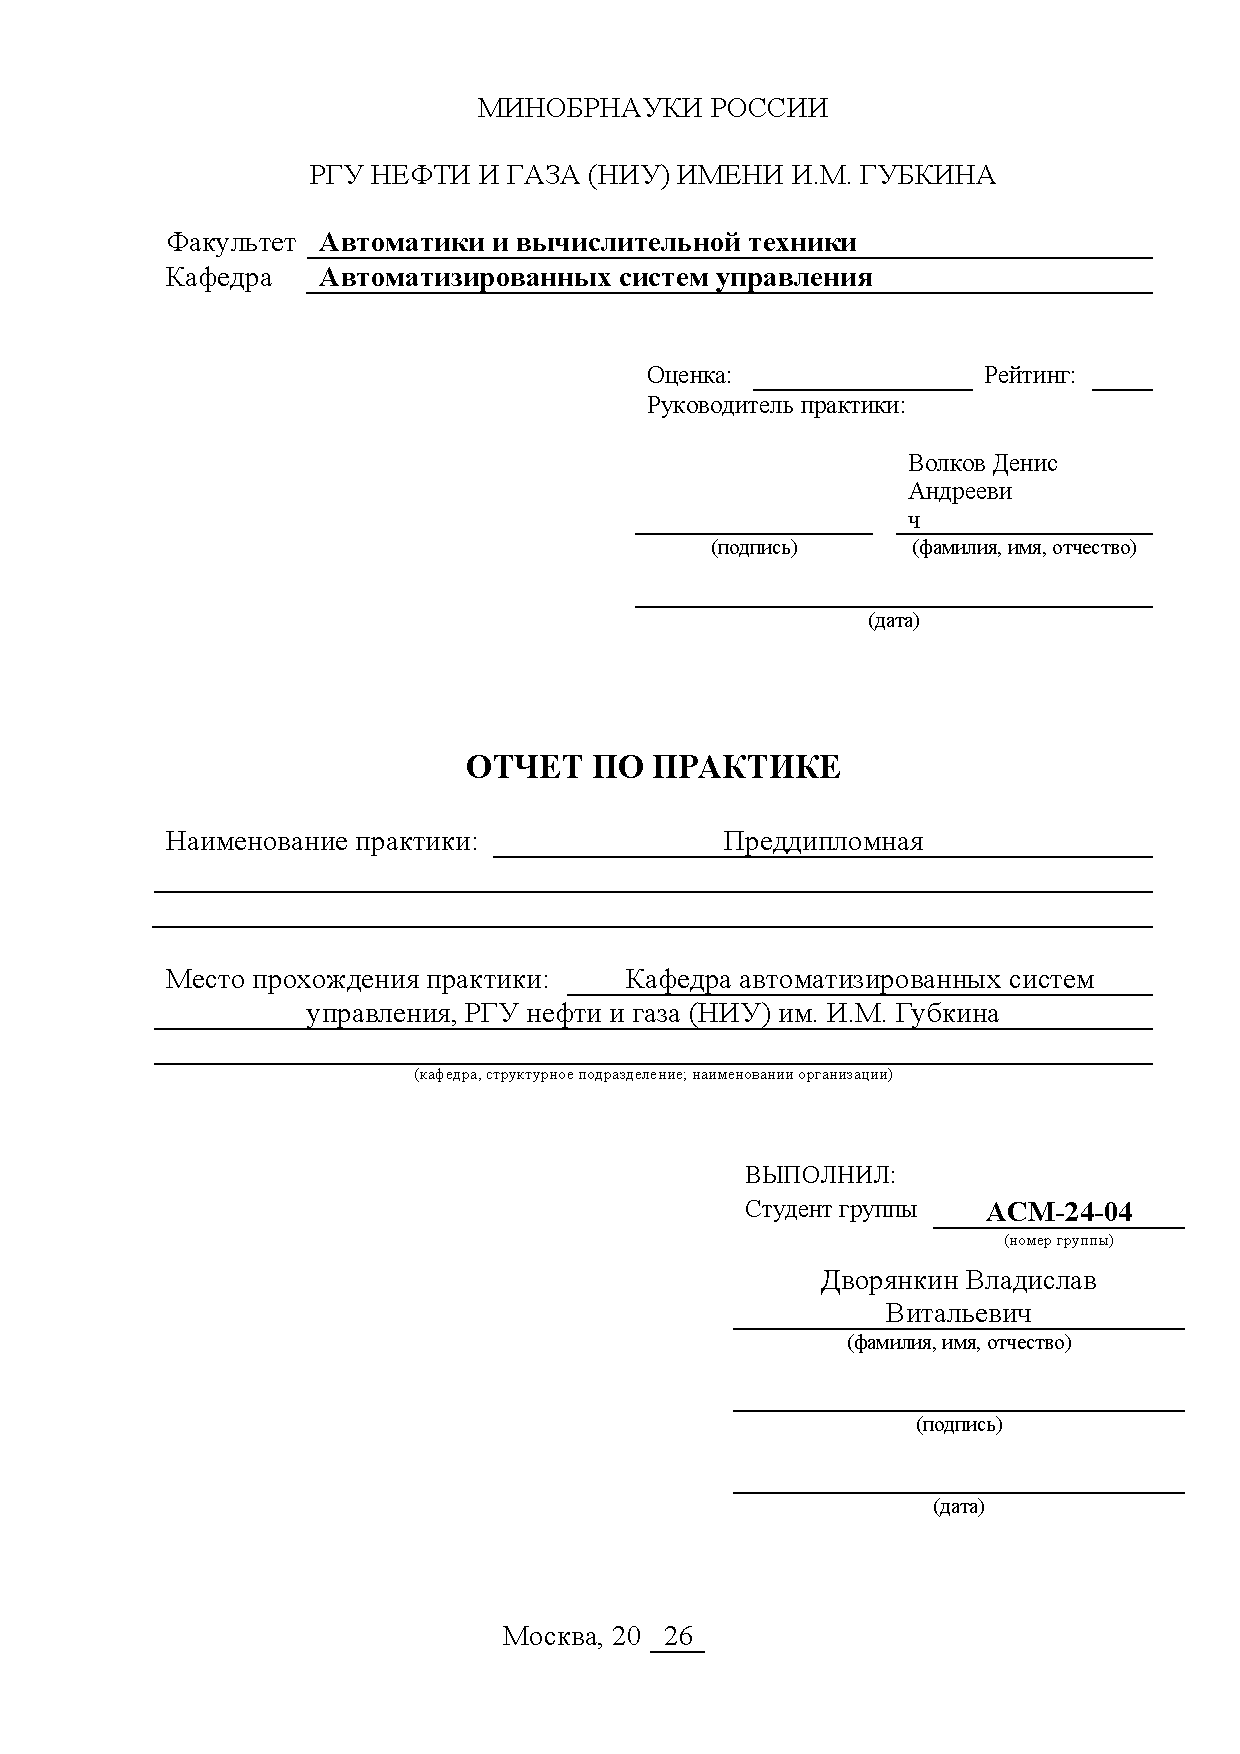
\includepdf[pages=-]{titulnik_praktika.pdf}

%%%%%%%%%%%% Оглавление %%%%%%%%%%%%%
\tableofcontents
\newpage

%%%%%%%%%%%% Введение %%%%%%%%%%%%%
\section*{Введение}
\addcontentsline{toc}{section}{Введение}

Современный учебный процесс в университете требует оперативной обратной связи между преподавателем и обучающимися непосредственно в ходе занятия. Для этого применяются интерактивные обучающие платформы. Существующие массовые решения --- Quizlet, Kahoot!, Mentimeter, Slido, JoyTeka, OnlineTestPad --- обеспечивают часть требуемой функциональности, однако ни одно из них не сочетает одновременно поддержку русского языка, развёртывание в инфраструктуре Российской Федерации, индивидуальное интервальное повторение учебного материала и психометрическую оценку качества тестовых заданий. Для регулярного применения на кафедре университета такого инструмента в настоящее время нет.

В связи с этим в рамках выпускной квалификационной работы разрабатывается программный сервис \emph{EduQuiz} для интерактивного взаимодействия с обучающимися. Сервис ориентирован на регулярное применение на кафедре университета и совмещает синхронные интерактивные сессии с игровой прогрессией, индивидуальное интервальное повторение по алгоритму SM-2 и психометрический анализ банка вопросов на основе коэффициента $\alpha$ Кронбаха.

\textbf{Целью} преддипломной практики является выполнение выпускной квалификационной работы~--- разработки моделей и сервиса EduQuiz для интерактивного взаимодействия с обучающимися в инфраструктуре российского университета.

Для достижения поставленной цели в ходе практики решались следующие \textbf{задачи}:
\begin{itemize}[leftmargin=*,nosep]
    \item провести сравнительный анализ распространённых интерактивных обучающих платформ и сформулировать требования к разрабатываемому сервису;
    \item спроектировать архитектуру сервиса и обосновать выбор технологического стека;
    \item разработать модели и алгоритмы интерактивного взаимодействия~--- ролевую модель пользователей, модель учебной сессии, модель игровой прогрессии, алгоритм индивидуального интервального повторения и модель оценки качества тестового инструмента;
    \item реализовать программный сервис, развернуть его в инфраструктуре Yandex Cloud, провести функциональное и нагрузочное тестирование;
    \item подготовить материалы к защите выпускной квалификационной работы.
\end{itemize}

\newpage

%%%%%%%%%%%% Описание работ %%%%%%%%%%%%%
\section*{Описание работ}
\addcontentsline{toc}{section}{Описание работ}

В ходе преддипломной практики при работе над выпускной квалификационной работой достигнуты следующие результаты:
\begin{itemize}[leftmargin=*,nosep]
    \item проведён сравнительный анализ шести распространённых платформ интерактивного обучения (Quizlet, Kahoot!, Mentimeter, Slido, JoyTeka, OnlineTestPad) и сформулированы требования к собственному сервису;
    \item спроектирована монолитная клиент-серверная архитектура; обоснован технологический стек: язык Go~1.25 с фреймворком Gin для серверной части, СУБД PostgreSQL~16, сервер кеширования Redis, клиентское приложение на Flutter Web, обратный прокси Caddy в качестве TLS-завершающего узла;
    \item разработаны модели и алгоритмы интерактивного взаимодействия: гибридная ролевая модель пользователей с разграничением доступа по схеме RBAC и дополнительной проверкой принадлежности ресурса; формальная модель интерактивной учебной сессии в виде конечного автомата; модель игровой прогрессии (очки опыта, бейджи, таблица лидеров); алгоритм индивидуального интервального повторения SM-2; модель оценки качества тестового инструмента на основе коэффициента $\alpha$ Кронбаха;
    \item реализованы четыре функциональных модуля сервиса (модуль аутентификации, модуль преподавателя, модуль проведения интерактивной сессии, модуль обучающегося), а также WebSocket-хаб событий для синхронной работы участников;
    \item настроена инфраструктура развёртывания на платформе Yandex Cloud: автоматизированная выкатка через GitHub Actions, автоматический выпуск сертификатов Let's Encrypt, накат миграций базы данных перед стартом приложения;
    \item проведено нагрузочное тестирование собственным программным инструментом (устойчивая работа при не менее 500 одновременных обучающихся в одной интерактивной сессии в одиночной серверной конфигурации) и функциональное тестирование, выполнена апробация на учебной группе.
\end{itemize}

Таким образом, в ходе практики разработан программный сервис EduQuiz для проведения интерактивных учебных сессий с поддержкой игровой прогрессии, индивидуального интервального повторения учебного материала и психометрической оценки качества тестовых заданий.

Также в ходе подготовки к защите выпускной квалификационной работы были созданы слайды презентации (рис.~\ref{fig:slide-01}--\ref{fig:slide-12}).

\begin{figure}[H]\centering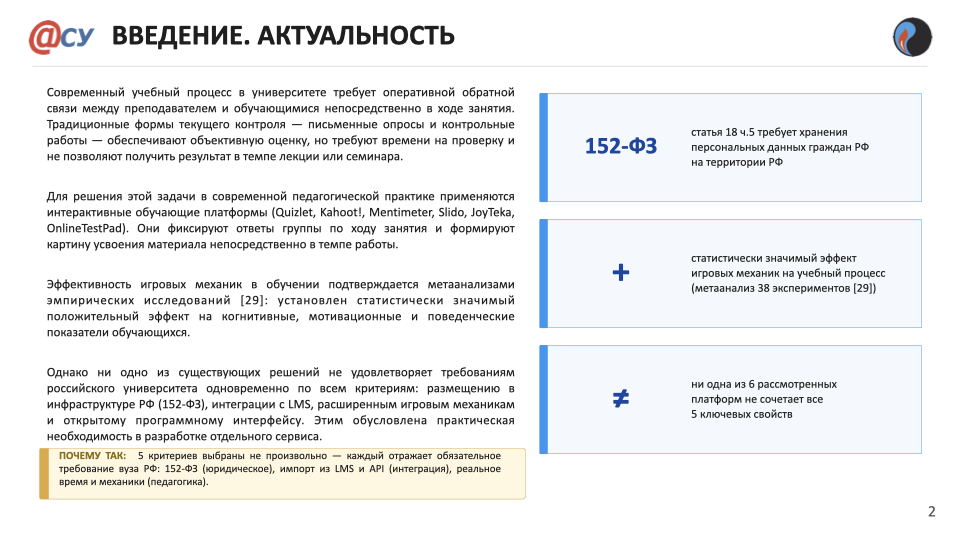
\includegraphics[width=0.92\linewidth]{slide-01.png}\caption{Слайд 1 <<Актуальность темы>>}\label{fig:slide-01}\end{figure}
\begin{figure}[H]\centering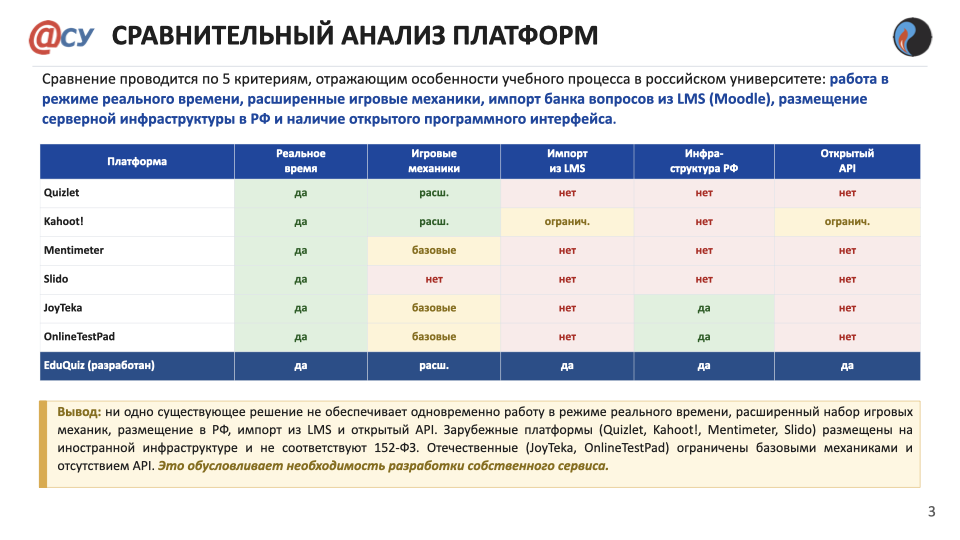
\includegraphics[width=0.92\linewidth]{slide-02.png}\caption{Слайд 2 <<Сравнительный анализ платформ>>}\label{fig:slide-02}\end{figure}
\begin{figure}[H]\centering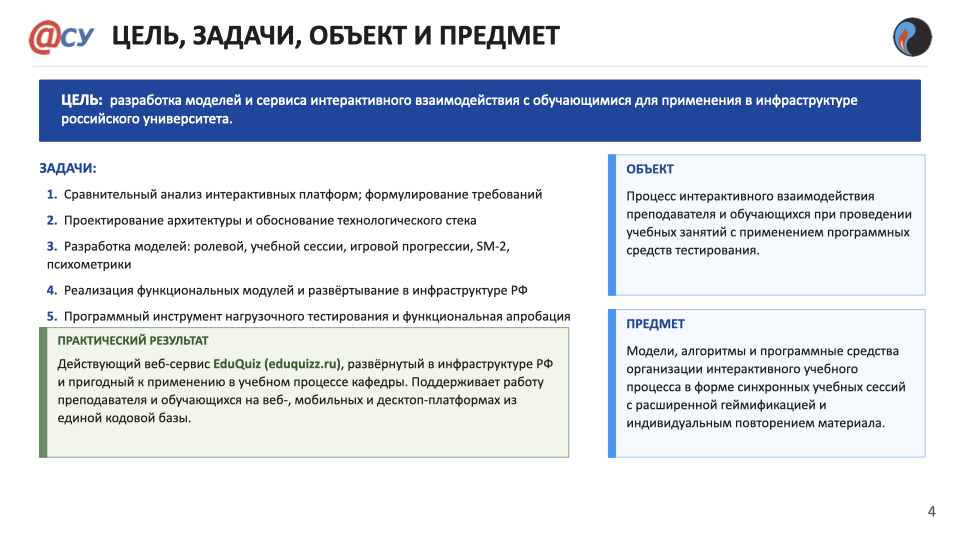
\includegraphics[width=0.92\linewidth]{slide-03.png}\caption{Слайд 3 <<Цель, задачи, объект и предмет>>}\label{fig:slide-03}\end{figure}
\begin{figure}[H]\centering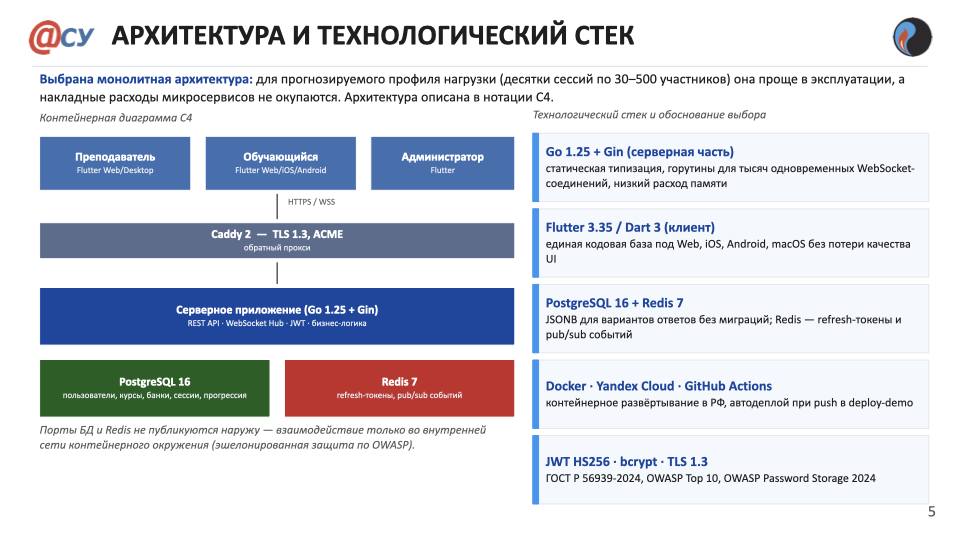
\includegraphics[width=0.92\linewidth]{slide-04.png}\caption{Слайд 4 <<Архитектура и технологический стек>>}\label{fig:slide-04}\end{figure}
\begin{figure}[H]\centering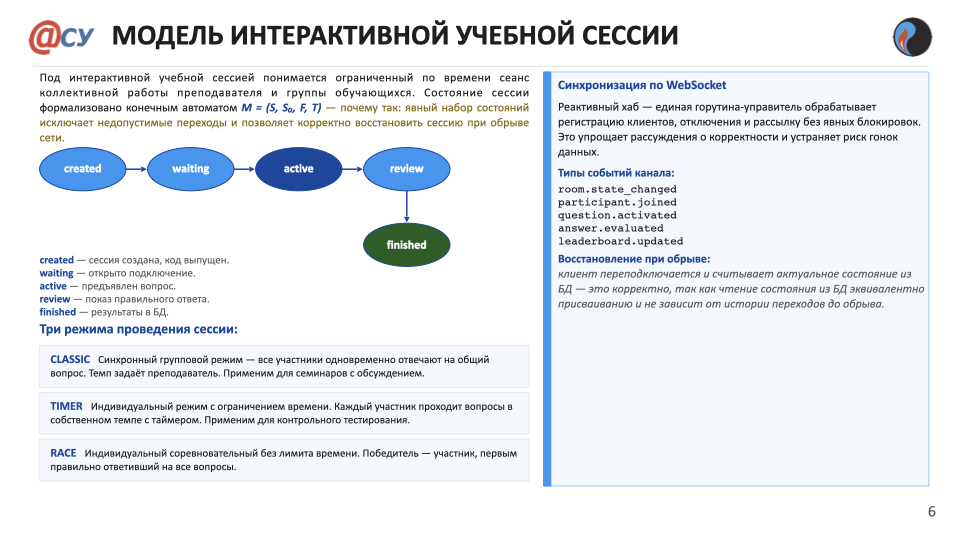
\includegraphics[width=0.92\linewidth]{slide-05.png}\caption{Слайд 5 <<Модель интерактивной учебной сессии>>}\label{fig:slide-05}\end{figure}
\begin{figure}[H]\centering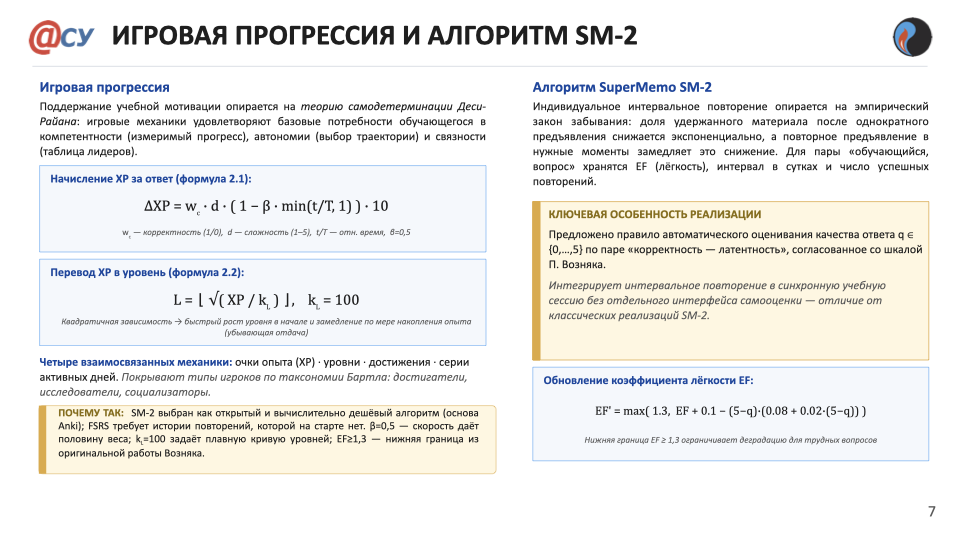
\includegraphics[width=0.92\linewidth]{slide-06.png}\caption{Слайд 6 <<Игровая прогрессия и алгоритм SM-2>>}\label{fig:slide-06}\end{figure}
\begin{figure}[H]\centering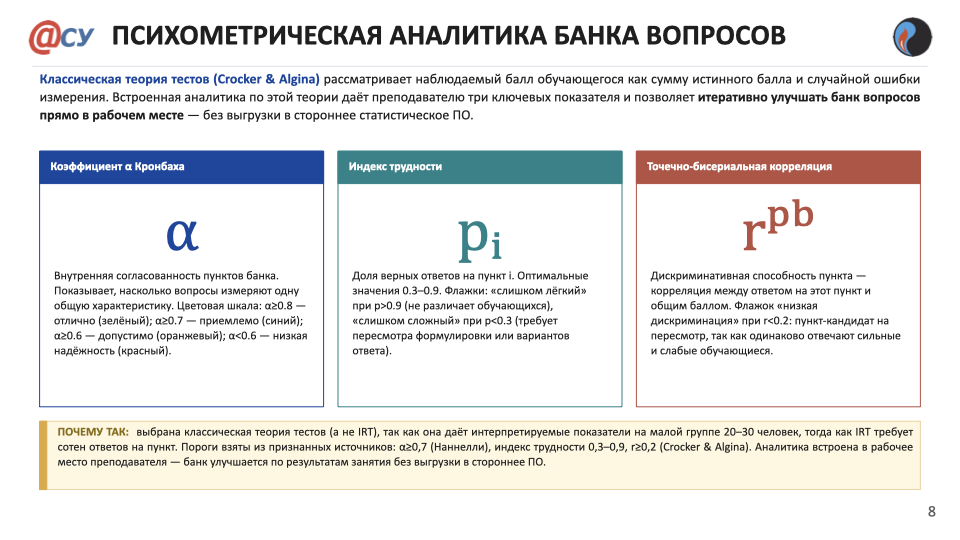
\includegraphics[width=0.92\linewidth]{slide-07.png}\caption{Слайд 7 <<Психометрическая аналитика банка вопросов>>}\label{fig:slide-07}\end{figure}
\begin{figure}[H]\centering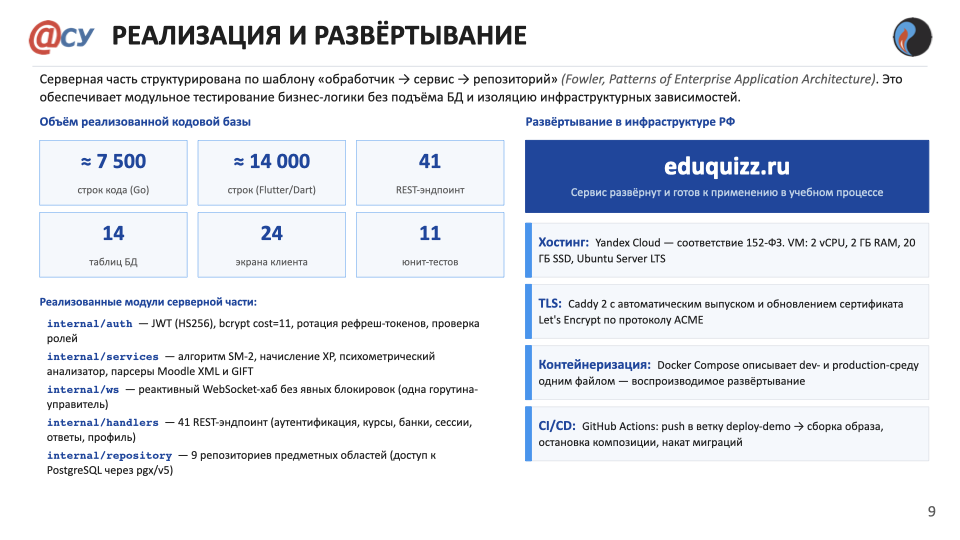
\includegraphics[width=0.92\linewidth]{slide-08.png}\caption{Слайд 8 <<Реализация и развёртывание>>}\label{fig:slide-08}\end{figure}
\begin{figure}[H]\centering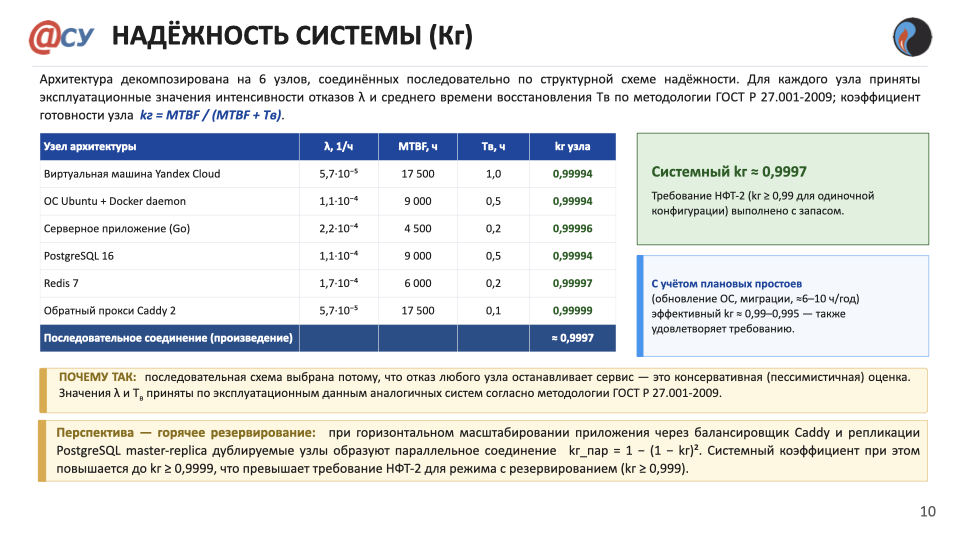
\includegraphics[width=0.92\linewidth]{slide-09.png}\caption{Слайд 9 <<Надёжность системы ($K_\text{г}$)>>}\label{fig:slide-09}\end{figure}
\begin{figure}[H]\centering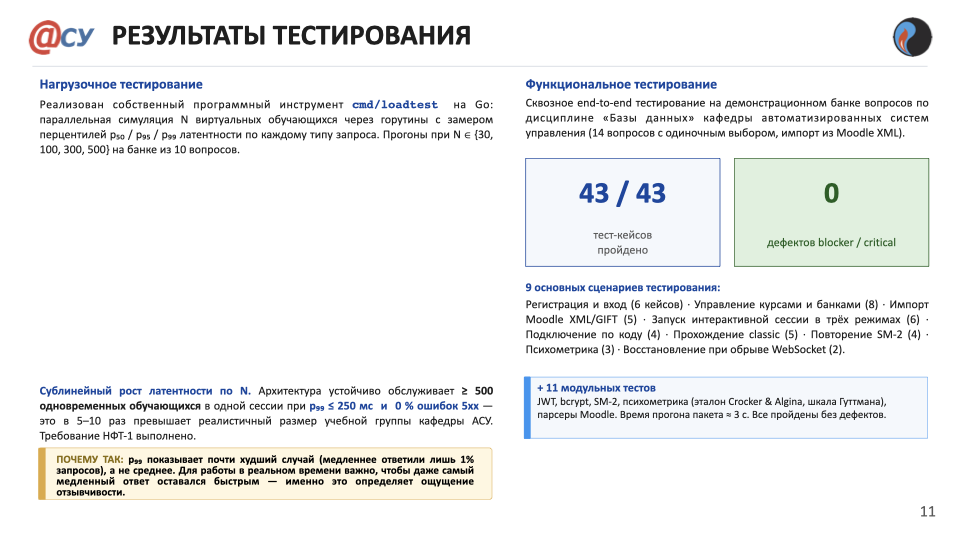
\includegraphics[width=0.92\linewidth]{slide-10.png}\caption{Слайд 10 <<Результаты тестирования>>}\label{fig:slide-10}\end{figure}
\begin{figure}[H]\centering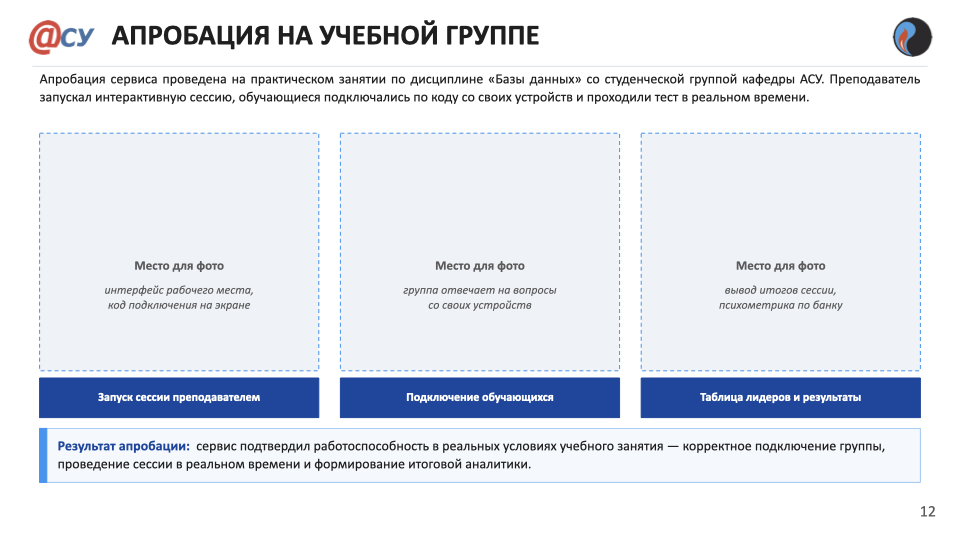
\includegraphics[width=0.92\linewidth]{slide-11.png}\caption{Слайд 11 <<Апробация на учебной группе>>}\label{fig:slide-11}\end{figure}
\begin{figure}[H]\centering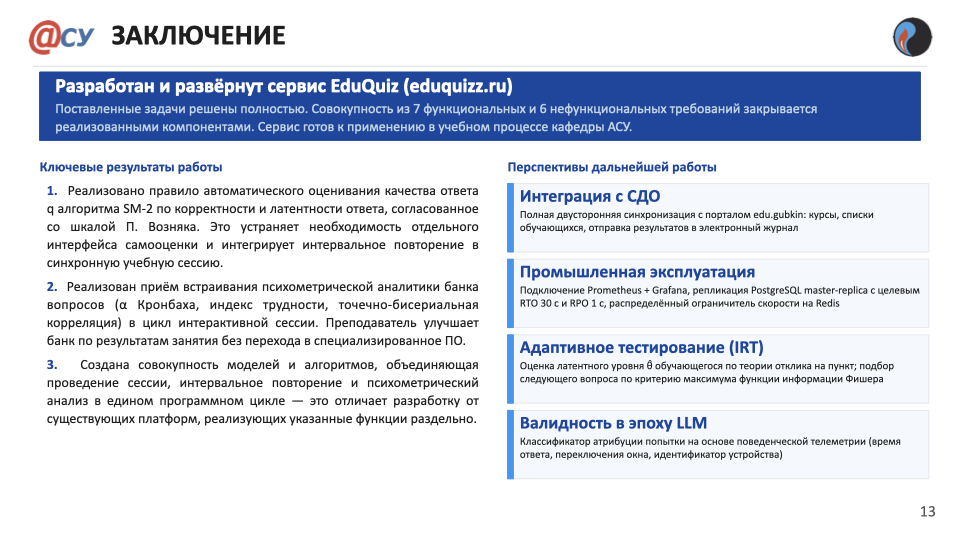
\includegraphics[width=0.92\linewidth]{slide-12.png}\caption{Слайд 12 <<Заключение>>}\label{fig:slide-12}\end{figure}

\newpage

%%%%%%%%%%%% Заключение %%%%%%%%%%%%%
\section*{Заключение}
\addcontentsline{toc}{section}{Заключение}

В ходе преддипломной практики был разработан программный сервис EduQuiz для интерактивного взаимодействия с обучающимися, развёртываемый в инфраструктуре Российской Федерации и применимый к преподаванию учебных дисциплин в университете.

В процессе работы изучены и применены: архитектурные подходы клиент-серверных систем; протокол WebSocket для синхронного взаимодействия участников; технологии аутентификации на базе JWT и подходы к защите от типовых угроз веб-приложений (OWASP Top~10); алгоритм индивидуального интервального повторения SM-2~(П.~Возняк); методы психометрической оценки качества тестовых пунктов на основе коэффициента~$\alpha$ Кронбаха; модели оценки надёжности систем (коэффициент готовности~$K_\text{г}$); инструменты автоматизированного развёртывания на базе Docker, Caddy, Let's Encrypt и Yandex Cloud.

По результатам нагрузочного тестирования собственным программным инструментом установлено, что разработанная архитектура в одиночной серверной конфигурации устойчиво обслуживает не менее 500 одновременных обучающихся в одной интерактивной сессии. По результатам функционального тестирования и апробации на учебной группе подтверждена работоспособность ключевых сценариев использования преподавателя и обучающегося.

Сформулированы \textbf{перспективы дальнейшей научно-исследовательской работы}:
\begin{itemize}[leftmargin=*,nosep]
    \item полная двусторонняя интеграция с системой дистанционного обучения университета (\texttt{edu.gubkin})~--- синхронизация курсов, списков обучающихся и выгрузка результатов;
    \item подключение промышленного мониторинга (Prometheus, Grafana, Alertmanager) и резервирование критичных узлов (репликация PostgreSQL, отказоустойчивая балансировка);
    \item эмпирическая калибровка параметров игровой модели (коэффициенты формулы начисления очков опыта) на репрезентативной выборке учебных групп;
    \item реализация адаптивного режима тестирования на основе теории отклика на пункт (IRT) с подбором сложности задания по текущей оценке способности обучающегося;
    \item исследование валидности атрибуции ответа в условиях широкого распространения общедоступных сервисов на основе больших языковых моделей.
\end{itemize}

\newpage

%%%%%%%%%%%% Список литературы %%%%%%%%%%%%%
\section*{Список литературы}
\addcontentsline{toc}{section}{Список литературы}

% Используется biblatex+biber + refs.bib (как в ВКР). Через \nocite
% подтягиваются нужные позиции; в самом отчёте инлайн-цитат нет.
\nocite{fz273,sagindykova2015,braude2020,sailer2020,koivisto2019,wozniak1990,cronbach1951,crocker_algina,kleppmann2017,gin_docs,postgresql_docs,flutter_docs,caddy_docs,gost25010}
\printbibliography[heading=none]

\end{document}
